% LaTeX mintafájl szakdolgozat és diplomamunkáknak az
% SZTE Informatikai Tanszekcsoportja által megkövetelt
% formai követelményeinek megvalósításához
% Modositva: 2011.04.28 Nemeth L. Zoltan
% A fájl használatához szükséges a magyar.ldf 2005/05/12 v1.5-ös vagy későbbi verziója
% ez letölthető a http://www.math.bme.hu/latex/ weblapról, a magyar nyelvű szedéshez
% Hasznos információk, linekek, LaTeX leirasok a www.latex.lap.hu weboldalon vannak.
%


\documentclass[12pt]{report}



%Az ékezetes betűk használatához:
\usepackage[T1]{fontenc}% ékezetes szavak automatikus elválasztásához
\usepackage[utf8]{inputenc}% ékezetes szavak beviteléhez

%Magyar nyelvi támogatás (Babel 3.7 vagy későbbi kell!)
%\def\magyarOptions{defaults=hu-min}
\usepackage[magyar]{babel}


% Margók és lap geometria beállítása
\usepackage{geometry}
\geometry{
  a4paper,
  %total={170mm,257mm},
  %left=2.5cm,
  top=2.5cm,
  %right=2.5cm,
  bottom=2.5cm
}

% A formai kovetelmenyekben megkövetelt Times betűtípus hasznalata:
\usepackage{times}

%Az AMS csomagjai
\usepackage{amsmath}
\usepackage{amssymb}
\usepackage{amsthm}

%A fejléc láblécek kialakításához:
\usepackage{fancyhdr}

%Természetesen további csomagok is használhatók,
%például ábrák beillesztéséhez a graphix és a psfrag,
%ha nincs rájuk szükség természetesen kihagyhatók.
\usepackage{graphicx}
\usepackage{psfrag}
\usepackage{xcolor}
\usepackage[hidelinks]{hyperref}

\usepackage{booktabs}
\usepackage{pifont}

%Tételszerű környezetek definiálhatók, ezek most fejezetenkent egyutt szamozodnak, pl.
\newtheorem{tet}{Tétel}[chapter]
\newtheorem{defi}[tet]{Definíció}
\newtheorem{lemma}[tet]{Lemma}
\newtheorem{áll}[tet]{Állítás}
\newtheorem{köv}[tet]{Következmény}

%Ha a megjegyzések és a példak szövegét nem akarjuk dőlten szedni, akkor
%az alábbi parancs után kell őket definiální:
\theoremstyle{definition}
\newtheorem{megj}[tet]{Megjegyzés}
\newtheorem{pld}[tet]{Példa}

%Margók:
\hoffset -1in
%\voffset 9.6mm%-1in % -25.4,,
%\oddsidemargin 35mm
%\textwidth 150mm
%\topmargin 15mm
%\headheight 10mm
%\headsep 5mm
%\textheight 237mm

\oddsidemargin 35mm%= 1cm




\begin{document}

%A FEJEZETEK KEZDŐOLDALAINAK FEJ ES LÁBLÉCE:
%a plain oldalstílust kell átdefiniálni, hogy ott ne legyen fejléc:
\fancypagestyle{plain}{%
	%ez mindent töröl:
	\fancyhf{}
	% a láblécbe jobboldalra kerüljön az oldalszám:
	\fancyfoot[R]{\thepage}
	%elválasztó vonal sem kell:
	\renewcommand{\headrulewidth}{0pt}
}

%A TÖBBI OLDAL FEJ ÉS LÁBLÉCE:
\pagestyle{fancy}
\fancyhf{}
\fancyhead[L]{Recipe hoarder webes alkalmazás}
\fancyfoot[R]{\thepage}


%A címoldalra se fej- se lábléc nem kell:
\thispagestyle{empty}

\begin{center}
	\vspace*{1cm}
	{\Large\bf Szegedi Tudományegyetem}

	\vspace{0.5cm}

	{\Large\bf Informatikai Intézet}

	\vspace*{3.8cm}


	{\LARGE\bf Recipe hoarder webes alkalmazás}
	\\\vspace*{0.3cm}
	{\Large\bf (Recipe hoarder web application)}


	\vspace*{3.6cm}

	{\Large Szakdolgozat}
	% vagy {\Large Szakdolgozat}

	\vspace*{4cm}

	%Értelemszerűen megváltoztatandó:
	{\large
		\begin{tabular}{c@{\hspace{4cm}}c}
			\emph{Készítette:}         & \emph{Témavezető:}      \\
			\bf{Vas Laura}             & \bf{Dr. Bilicki Vilmos} \\
			gazdaságinformatika szakos & egyetemi adjunktus      \\
			hallgató                   &
		\end{tabular}
	}

	\vspace*{2.3cm}

	{\Large
		Szeged
		\\
		\vspace{2mm}
		2021
	}
\end{center}


%A tartalomjegyzék:
\tableofcontents

%A \chapter* parancs nem ad a fejezetnek sorszámot
\chapter*{Feladatkiírás}
%A tartalomjegyzékben mégis szerepeltetni kell, mint szakasz(section) szerepeljen:
\addcontentsline{toc}{section}{Feladatkiírás}

A szakdolgozat során egy Angular keretrendszerben kialakított webes alkalmazás létrehozása volt a feladatom.
A projekt a Firebase-t használja adatbázisként. A fejlesztés során a legfőbb cél a recept importálás más honlapokról volt.
Az importálás második legfontosabb lépése az alapanyagok szétválogatása,
hogy később a bevásárlólistába helyezésnél a megyegyező anyagok összeadódjanak.

\chapter*{Tartalmi összefoglaló}
\addcontentsline{toc}{section}{Tartalmi összefoglaló}

\begin{itemize}
	\item téma megnevezése: \\
	      A szakdolgozat céljául kitűzött témám egy Angular-ban írt web applikáció, ami recept megjelenítésre és importálásra használható.
	\item feladat megfogalmazása: \\
	      Az importálás funkció lehetővé teszi, hogy a ˝ felhasználók egy helyen gyűjtsék a receptjeiket. Továbbá a regeptek összetevőit egy bevásárló listába ki tudják menteni, ezzel is megkönnyítve a mindennapi életet. A felhasználók a többiek által létrehozott receptek között tudnak keresni, és a nekik tetsző recepteket ki ˝ tudják menteni a saját receptgyűjteményeikbe.
	\item megoldási mód: \\
	      Az applikáció egy weblap formájában lett megvalósítva, mivel így lehet a legtöbb eszközt elérni egyetlen kód bázissal. A megvalósításhoz a már említett Angular keretrendszert használtam, illetve a Firebase felhő alapú szolgáltatásait. Mivel mind a kettő (Angular, Firebase) a Google terméke, ezért várhatóan hosszútávon támogatva lesznek. A felhasználó a recept URL-je alapján tud, receptet importálni, vagy manuálisan is tud létrehozni újat. Ekkor az importáláshoz egy szerver oldali funkció fut le és próbálja értelmezni a megkapott URL-en lévő html fájlt. Ennek egy fontos lépése az, hogy az alapanyagok nevét, mértékegységét és mennyiségét az eredeti kiolvassa. Ehhez regex-et illetve egy külső konyvtárat használtam, ami sok mértékegység között tud átváltani. Miután a receptet sikeresen importáltuk, azokat a Firebase FireStore adatbázisában tároljuk.
	\item alkalmazott eszközök, módszerek: \\
	      Mind az importálás mind az egész projekt során törekedtem, hogy minél modulárisabb legyen a felépítés. A webapp fejlesztése során a PWA-t alkalmazva elérhető, hogy ˝ bizonyos funkciók offline is működjenek. A modern, könnyen kezelhető weblap számítógépen és telefonon egyaránt használható.
	\item elért eredmény: \\
	      A fejlesztés során sikerült egy modern telefonos és számítógépes környezetben is elérhető webes alkalmazást készíteni, ami bárki számára a regisztráció után elérhető és könnyen használható, ezzel könnyebbé téve a hétköznapokat.
	\item kulcsszavak: \\
	      Angular, Firebase, pipeline architektúra, PWA, telefonos nézet
\end{itemize}

%Bevezetés
\chapter*{Motiváció}
\addcontentsline{toc}{section}{Motiváció}

Egyetemisták, mint én is egyre közelebb vagyunk ahhoz az életformához, ahol önellátók vagyunk, ennek fontos része a főzés és étkezés. Manapság nagyon egyszerű különböző recepteket, különböző országokból, kultúrákból találni, viszont ez temérdeknyi weblapot jelenthet. Ennek hátulütője, hogy egy idő után követhetetlen lesz, hogy egyáltalán hova regisztráltunk, valamint, hogy “melyik weblapon is volt az a bizonyos recept, amit egyszer már kipróbáltam, és tetszett”. Személyes tapasztalatom ezzel kapcsolatba pedig, hogy én egy TXT fájlba mentegettem az URL címeket, hogy legközelebb is megtaláljam, de már kezdett nagyon követhetetlen lenni.

Azért választottam ezt az ötletet a szakdolgozatom témájának, mert ez egy személyes problémám már hosszú ideje és láttam már korábban próbálkozásokat, de egyik sem volt az én elképzelésemnek megfelelő. A célom az volt, hogy egy egyszerű URL cím másolással pillanatok alatt egy helyen lehessen a megtalálni mindent.

A továbbiakban részletesen részletezem az általam tervezett és megvalósított webes applikáció felépítését és funkcióit. A bemutatót a konkurencia ismertetésével kezdem.


\chapter{Piacfelmérés}
Már létező programokra öt példát hoztam, amik mind valamilyen szinten különböznek.
Felhasználó körük, funkcióik, előnyök és hátrányok az én tervemhez képest.

\section{Grocy}
A Grocy egy lokálisan hostolható weblap. Irgalmatlanul részletes és rengeteg funkciója van, amihez, ha az ember hozzászokik és elég időt és törődést fektet bele, akkor egy nagyon hasznos program. Ellenben, mivel lokálisan van felépítve, ezért, ha valaki most kezdené el először használni, akkor nagyon sokáig tart, amíg igazán használható lehet.

A recept kezelő lapja csak manuálisan feltölthető, tehát nincs importálásra lehetőség. Rendelkezik bevásárlólista és “sufni” opciókkal is. Az otthon lévő alapanyagokat egyessével, tetsző részletességgel fel lehet venni a “sufniba”, ezzel leltározva, hogy milyen alapanyagok vannak otthon. Ezekről eltárolható adatok közé tartozik, hogy mennyi van belőle, meddig jók, képet, de akár a vonalkódját is. A bevásárló lista pedig egyértelműen a vásárlást segítő funkció, aminek a végén, egy kattintásra átrakható “sufniba”.

Már ezen kis leírás alapján is látszik, hogy ahhoz, hogy ez a rendszer használható legyen, egy komoly lokális adatbázist kell létrehozni az alapanyagokból és azok adatairól, valamint a receptekről. Ez a rendszer csak limitált tudású emberek számára használható, mivel már csak a telepítése is kicsit bonyolultabb, ezért átlag emberek számára nem ajánlott.

\section{Delish}
Ezt a weblapot azért választottam példaként, mert ez egy tökéletes példa egy átlagos, egyszerű receptes weblapokra.  A honlapon csak recepteket és talán pár blog bejegyzés található regisztráció után is. Ez a weblap reprezentálja a legtöbb hasonló, csak blogként működőket.

Egy receptre kattintva látjuk az alapadatokat, hozzávalókat, elkészítési javaslatot valamint alap adatokat mint az elészítési idő. A weblaon található még hasonló recept ajánlások, de ezzel le lett fedve minden funckciója.

\section{Yummly}
Ez egy fejlettebb verziója a korábban említett "átlagos" weblapoknak. Bejelentkezés nélkül egy kissé korlátolt, viszont utána már kifejezettem sok képessége van. A webes kinézeten felül applikációval is rendelkezik.

Az alap recept keresésen kívűl, itt már lehetőségünk van azok elmentésére a sajátjaink közé. A weblap rendelkezik bevásárló lista funkcióval, valamint képes azonnal a receptből áthelyezni az alapanyagokat is. Egy kiemelkedő funkciója az étkezés tervező. Ez, figyelembe véve esetleges allergiákat, vagy étrendeket ajánj és segít tervezni a következő időszakra.

Ami hátrány az egész weblapon, hogy nem közösség bővíti a recept adatbázist, ezért limitált a receptek száma és nem lehet mindent megtalálni. Még akkor is, ha figyelembe vesszük a manuális recept készítést, nem feltétlenül a leg felhasználóbarátibb, hogy mindig egy külső helyről egyösször kikeressük amit akarunk, majd kézzel beírjuk.

\section{BigOven}
A legnagyobb különbség az eddigiekhez képes, hogy ez a weblap már rendelkezik recept importáló funkcióval is. Azon felül négy különböző módon lehet újjakat létrehozni. Az importálás során nem tárolják el az egész receptet, ha más honlapról származik. "Our Pledge to Food Bloggers" leírja, hogy miért, viszont ez azt jelenti, hogy a teljes receptet megtekintsük, át kell navigálni az eredeti oldalra. Ezen felül a bevásárló listában nem adódnak össze a termékek, valamint nincsenek kategóriák a receptekhez.

Egy nagy hátránya a weblapnak, hogy kissé régi stílusú. A gombok majdnem eredeti HTML alakban jelennek meg. A képek, form-ok, lista nézet mind úgy néz ki, amin épphogy van egy kis formázás. A webes kinézenket a navigációja nem a leg felhasználóbarátibb.

Annak ellenére, hogy a weblapnak mennyire nem modern stílusa van, az applikáció igenis követhető. A funkciók szintén jól működnek. Elméletileg IOS-en is létezik, viszont arra nincs lehetőségem, hogy felmérjem milyen különbségek lehetnek. Egy nagy előny, hogy az ingyenes verzióban is használhatóak az alapfunkciók.

\section{ChefTap}
Az összes közül valőszínűleg ez az applikáció, ami a legtöbb funkcóval rendelkezik. Technikailag van webes és telefonos applikációs verziója is, viszont a webes csak recept lekérdezésre használható. Minden egyéb, beleértve a recept importálást, bevásárló listát, étkezés tervezőt csak az applikációk keresztűl lehet elérni és szerkeszteni. A weben volt lehetőség Google segítségével bejelentkezni, viszont az applikációnak nem volt ilyen lehetősége. Ennél az appnál az ingyenes verzió elég limitált, a recept importáláson kívül semmi sem működik a próbaidőszak lejárta után.

Ezen a felületen nincs mások által, vagy akár csak egy közös adatbázisból való keresésre és importálása lehetőség a recepteknél. A felhasználónak mindent magának kell beszerezni.

A beimportált recepteket könnyű módosítani, valamint rengeteg kis adatot megadni, hogy otthonosan lehessen használni a környezetet. Itt nincs lehetőség közvetlenül a receptből a bevásárló listába rakni alapanyagokat, menüket összekészíteni vagy az étkezéstervezőt használni az ingyenes próbaverzió után.

\section{Összefoglaló}
Egy táblázat a korábban összefoglalt példákról és tudásaikról egy egyszerű összehasonlításhoz.

\newcommand{\cmark}{\ding{51}}%
\newcommand{\xmark}{\ding{55}}%

\noindent
\begin{tabular}{p{3cm} | c c c c c | c @{}}
	\multicolumn{7}{c}{Összegzés}                                                                   \\ \midrule
	weblapok                         & Grocy  & Delish & Yummly & BigOven & ChefTap & RecipeHoarder \\ \cmidrule[2pt](r){2-7}
	open source                      & \cmark & \xmark & \xmark & \xmark  & \xmark  & \xmark        \\\cmidrule(r){2-7}
	recept importálás - URL          & \xmark & \xmark & \xmark & \cmark  & \cmark  & \cmark        \\ \cmidrule(r){2-7}
	receptekhez vannak lépések       & \xmark & \cmark & \cmark & \xmark  & \cmark  & \cmark        \\ \cmidrule(r){2-7}
	manuális recept hozzáadás        & \cmark & \xmark & \xmark & \cmark  & \cmark  & \cmark        \\ \cmidrule(r){2-7}
	bevásárlólista                   & \cmark & \xmark & \cmark & \cmark  & \cmark  & \cmark        \\ \cmidrule(r){2-7}
	bevásárlólista ajánló            & \cmark & \xmark & \xmark & \xmark  & \xmark  & \cmark        \\ \cmidrule(r){2-7}
	katgóriák használata receptekhez & \xmark & \cmark & \cmark & \xmark  & \cmark  & \cmark        \\ \cmidrule(r){2-7}
	étkzés tervező                   & \cmark & \xmark & \cmark & \xmark  & \xmark  & \xmark        \\ \cmidrule(r){2-7}
	bejelentkezés google fiókkal     & \xmark & \cmark & \cmark & \cmark  & \xmark  & \cmark        \\ \cmidrule(r){2-7}
	reszponzív weblap                & \cmark & \xmark & \xmark & \xmark  & \xmark  & \cmark        \\ \bottomrule
\end{tabular}

\chapter{Funkcionális specifikáció}
Egy összefoglaló részletesebb arról, hogy minek pontosan hogyan kell működnie az eredeti terv szerint. \\

\noindent
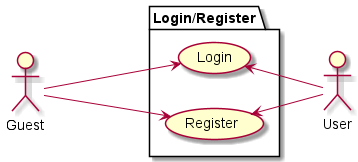
\includegraphics[scale=0.6]{out/diagrams/useCaseGuest/useCaseGuest.png} \\
\noindent
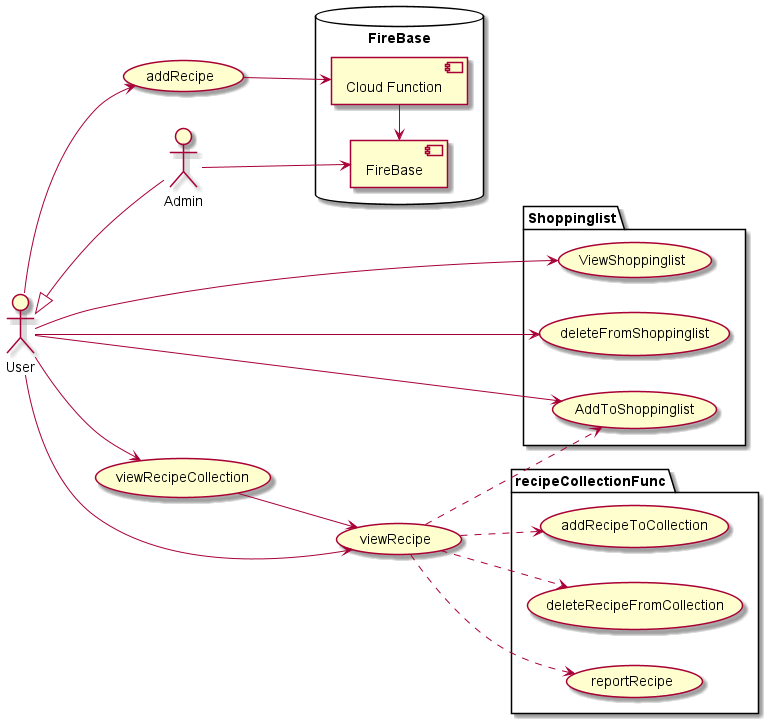
\includegraphics[scale=0.5]{out/diagrams/useCaseUser/useCaseUser.png}


\section{Bejelentkezés/Regisztráció}
A regisztrációt és bejelentkezés a legbiztosabb biztonság érdekében a Firebase Auth rendszerén keresztül történik. Kettő módszer van a regisztrációra. Első, a szokásos email és jelszó páros megadásával a regisztrációs formon keresztül. Második, a Google authentikációs rendszeren keresztül. A felhasználók ezt látják először, mikor a honlapra navigálnak. Bejelentkezés nélkül nem lehetséges a weblapot megtekinteni.
\noindent
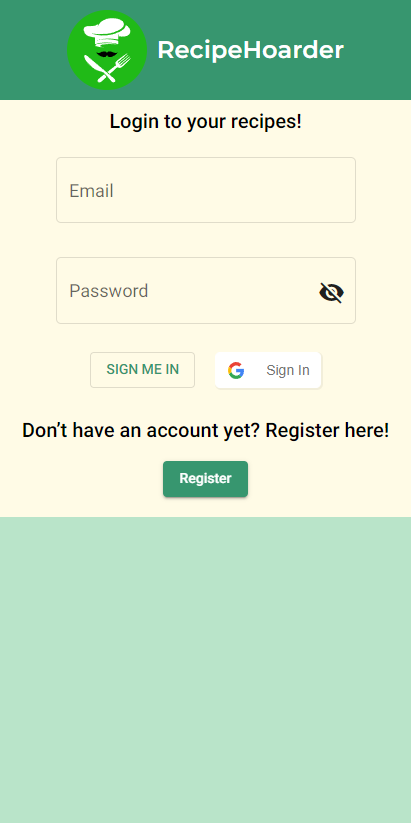
\includegraphics[scale=0.5]{pictures/mobil_login.png}
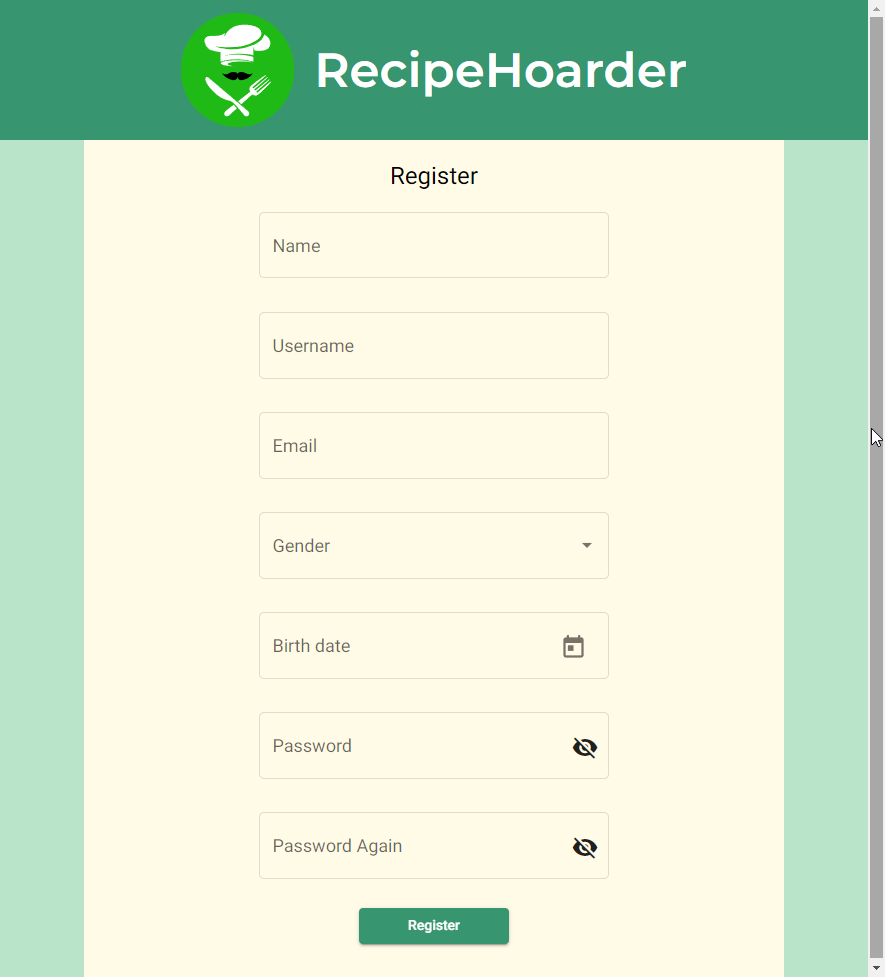
\includegraphics[scale=0.4]{pictures/web_register.png}

\section{Kezdőoldal}
A kezdőoldalnak az első lap, amit a bejelentkezés után látnak a felhasználók. A lapon két különböző recept ajánló jelenik meg. Az egyik a saját, kimentett receptekből ajánlott fel párat, a másik viszont a még nem kimentett receptekből. Ezen felül a kategória keresés is itt érhető el. Minden receptnek létrehozáskor kötelezően van legalább egy kategóriája, ezért ez a típusú keresés jó az általános recept felfedező felhasználóknak.
\noindent
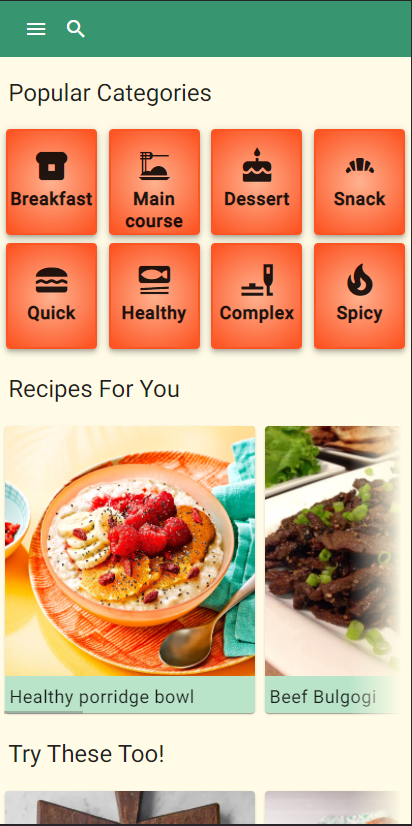
\includegraphics[scale=0.5]{pictures/mobil_home.png}

\section{Recept saját gyűjteményekbe}
A létező recepteknél a megnyitás után egy gombnyomással lehetőségünk van azt a saját gyüjteményünkhöz adni. Amennyiben ez sikerült, a gomb átváltozik egy kuka ikonra. Ez újonnan megnyomása után a recept kikerül az elmentettjeink közül. Ez a lista egyszerűen megtalálható az oldal menüben a "My recipes" alatt. Ezen lap alatt az összes korábban elmentett recept kilistázódik.

Amennyiben a felhasználó kimentett egy receptet, a törlés gombra változásán kívül egy szívecske is megjelenik a recepten. Erre nyomva a recept egy külön listába kerül, ahol a saját receptek közül csak a kedvenceket lehet gyorsan eltárolni. A szivecskére kattintással ki és be lehet kapcsolni, hogy a kedvencek közé kerüljön. Amint a felhasználó ki veszi a receptet a saját gyűjteményéből, akkor a kedvencek közül is eltűnik. A lista megtalálható az oldalsó menüben a "My favourites" menüpont alatt.
\noindent
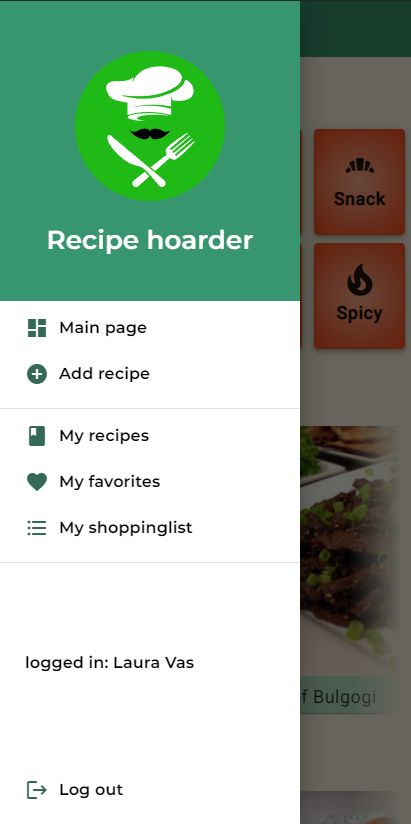
\includegraphics[scale=0.5]{pictures/mobil_menu.png}
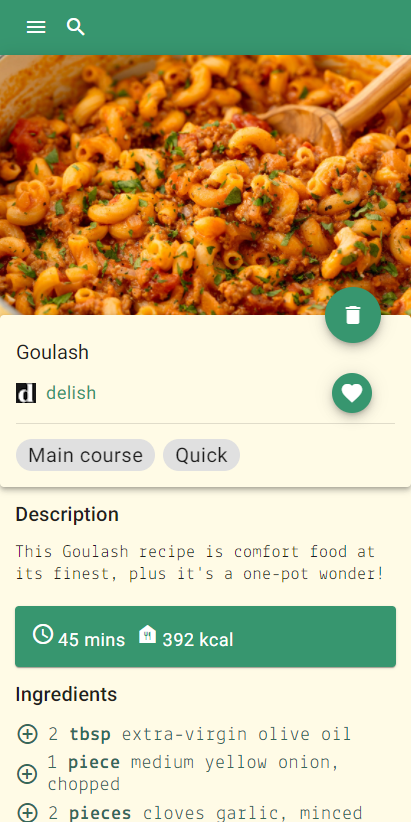
\includegraphics[scale=0.5]{pictures/mobil_recipe-top.png} \\
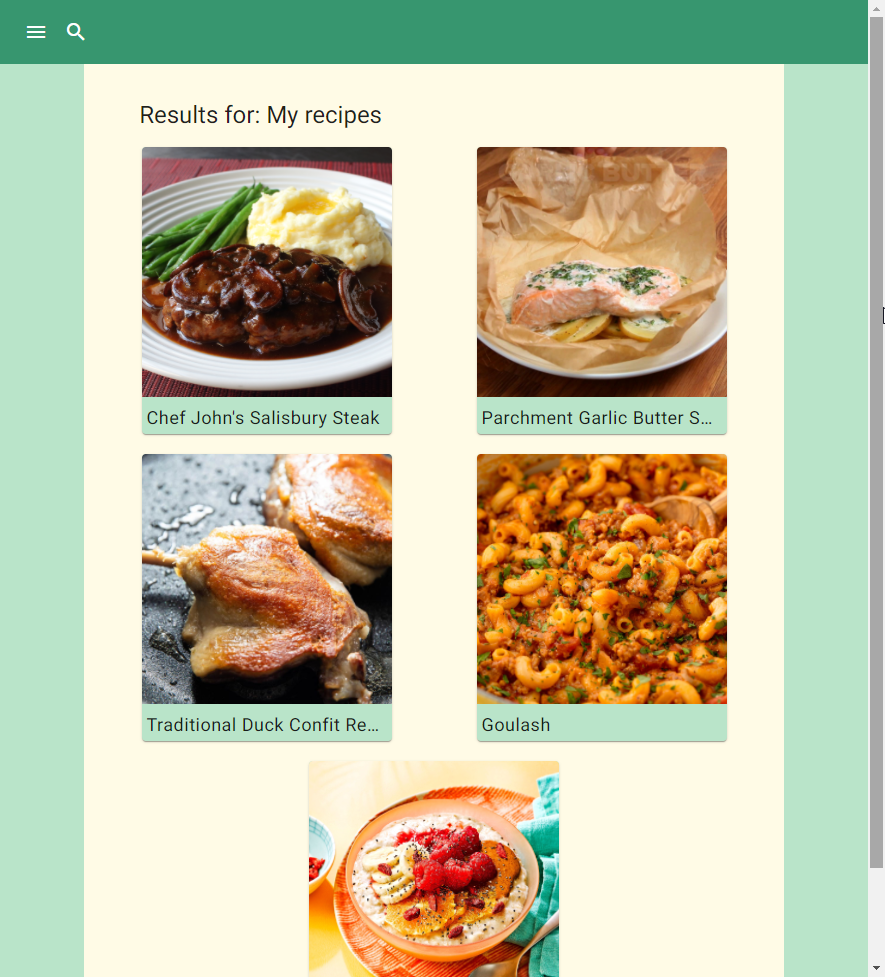
\includegraphics[scale=0.4]{pictures/web_recipeCollection.png}

\section{Recept importálás}
Két féle képpen lehet recepteket létrehozni. Az elsőnél a felhasználónak csak ki kell tölteni a mezőket az új recept létrehozó felületen. Az alapanyagokból és lépésekből tetsző mennyiséget tud létrehozni, valamit törölni is.

A második módszer, ami a korábbi folyamat megkönnyítse miatt jött létre, a recept importálás URL-en keresztül. A felhasználó csak kiválaszt egy receptet egy másik honlapról, kimásolva az URL címét és az importálás folyamat során egy Cloud Function lekérdezi az adatokat. A funkció modulásisan lett felépítve, ezért jobban követhető, valamint bővíthető. Az importálás fontos része az alapanyagok szétválasztása alapanyag mennyiség, mértékegység és név szerint. Ez a receptnézetnél is megjelenik, de a fő célja a kalóriaszámlálásnál és a bevásárló listába helyezésnél kerül elő. A lekérdezés során, az egyik modul feladata a képek mentése az eredeti helyről, valamint feltöltése a Firebase Storage-ba. Ez fontos lépés,mert ha a weblap vagy recept egy ponton megszűnne, akkor is megmarad a  kép és adatok a receptről. Amint a funkció lefutott, egy új lapra át lesz navigálva a felhasználó, ahol a recept szerkeszthető mezőkben megjelenik, ilyenkor még nincs elmentve az új adat az adatbázisba. Az importálás sikerességének átvizsgálása után, a felhasználó nyomhat a véglegesítő gombra.

A manuális és URL-es importálás ugyanazon a lapon működik, az egyetlen különbség, hogy üresen jut-e oda, vagy már lehetőleg egy sikeres lekérdezés után egy feltöltött verzióra. A véglegesítés előtt viszont, ha a felhasználó még nem választott besorolási kategóriát, akkor egy felugró ablak figyelmezteti, hogy ezt mindenképp tegye meg, mert nem léphet tovább anélkül.\\

\noindent
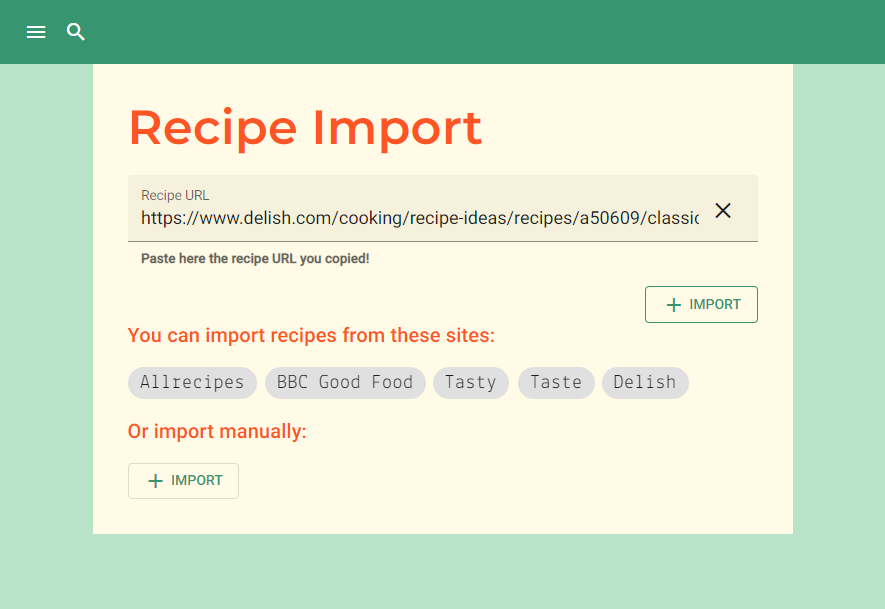
\includegraphics[scale=0.4]{pictures/web_import.png}
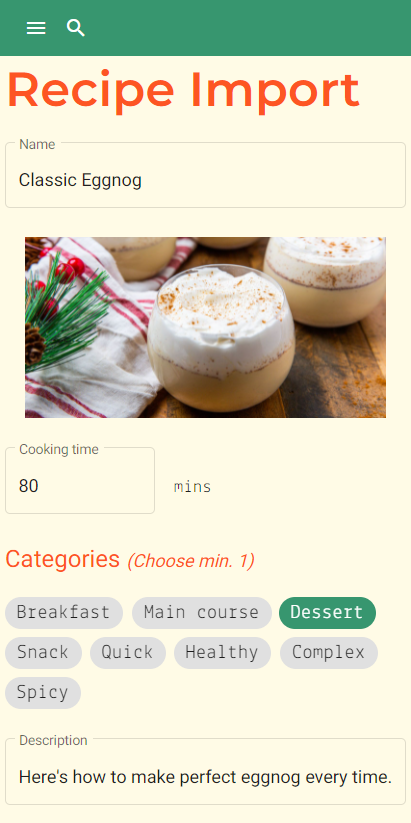
\includegraphics[scale=0.5]{pictures/mobile_importDataCheck.png}

\section{Recept kalória számlálás}
Ez a lépés egy modul a recept importálás folyamatban. A projekthez hozzáadtam egy csomagot, ahonnan egyrészt a szétválasztáshoz megkapom a mértékegységeket, másrészt ezt használom a mértékegység átváltáshoz is. 

A tápanyag információkat egy külső adatbázisból szedem, ami az amerikai állami  Food Data Central API-ból elérhető. A használati feltételeket végigolvasva kiderült, hogy bárki ingyen használhatja, akár a jogok feltüntetése nélkül is, bár megköszönik, amennyiben ez feltűntetve lesz. Csak regisztrálni kell a weblapon ahhoz,hogy saját API kulcsot kapjunk.

A kalóriaszámlálás kizárólag akkor fut le, ha a receptlekérdezés során nem létezett az eredeti oldalon a kalória információ, vagy ha a recept manuálisan lett létrehozva. Ahhoz, hogy megfelelő eredményt kapjunk legalább 80 százaléknyi kiszámolt kalória adatok kell visszakapni az eredeti alapanyag mennyiségéhez képest. Ha ez nincs meg, akkor nem lesz megjelenítve kalória információ a recepthez. Amennyiben megfelelő mennyiségű adatunk van, a korábban említett mértékegység átváltásokkal egységesítem az alapanyagokat a tápanyag táblázat értékéhez, aztán azt összeadva kapjuk a kalória adatot a recepthez.

\section{Bevásárlólista}
A bevásárlólista egy külön lapon található, ahol a felhasználó a saját vásárlásához gyűjthet alapanyagokat. Ha a lapon található új alapanyag hozzáadó felületet használja, akkor hozzáadás után azonnal, megjelenik a leni listában az új elem. Ha  listában még létezett egy ponosan olyan nevű elem, akkor, ha szükség van rá, egy mértékegység átváltással hozzáadódik az eredeti elemhez. Így az alapanyag mennyisége nő. Amennyiben nem kell már az alapanyag, a sor végén lévő pipával ki lehet venni a listából.

A felhasználó kényelme érdekében, a receptből közvetlenül az alapanyag előtti plusz gombra nyomva hozzá lehet adni egyesével az alapanyagokat a bevásárló listába. Valamint ha mindent gyosan hozzá szeretnénk adni, akkor van egy másik gomb az alapanyag lista alatt,amivel az összeset egy kattintással hozzá lehet adni a listához.\\

\noindent
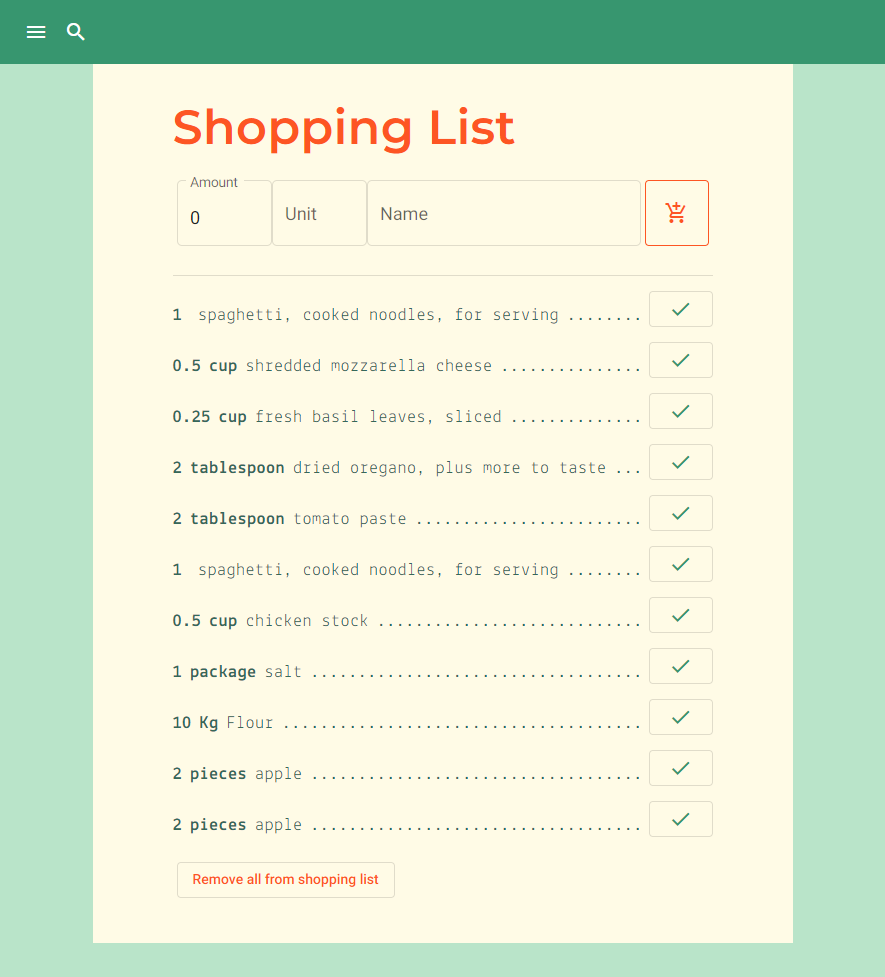
\includegraphics[scale=0.4]{pictures/web_shoppinglist.png}

\section{Bevásárlólista ajánló}
A bevásárló listát használó felhasználók a lista megnyitásakor kapnak egy felugró lista elemet, ami egy korábbi alapanyagot kínál, amennyiben az több mind egyszer lett a listához adva. A pipára nyomva, az alapanyag bekerül a hozzáadó mező név elemébe. Amint a mennyiséget és mértékegységet kitöltve hozzáadjuk, akkor egyrész hozzáadódik az új elem a listához, valamint a következő alkalom dátuma újra generálódik a korábbiakat átlagolva.

Amennyiben a felhasználót nem érdekli az ajánlat, az x-re nyomva az ajánlat eltűnik, valamint elindul a funkció, ami -1 értékkel levonja az ajánlat értékelését. Az értékelés mező értéke alapvetően 2 mikor létrejön a meta adat. Amint az érték eléri a nullát, az alapanyag nem lesz többször felajánlva egy ideig.

	{\color{green}{
			\verb!Lehet, hogy ez már specifikáció inkább...!\\
			Annak érdekében, hogy ha a felhasználó egy ideig elvetette az alapanyagot, de egy idő után az mégis sokszor újra bekerül a listába, akkor minden hozzátételnél az értékelés mező +0.1 értékkel nő, ami lehetővé teszi, hogy egy idő után visszakerüljön az ajánlottak közé.

			Az ajánlás egy sima adatbázis lekérdezés, ami szűrve van úgy, hogy csak ez a pillanat előtti “ajánlott időpont”-os alapanyagokat kérdezzünk le, ami rendezve van dátum és értékelés csökkenő sorrendjében. Végűl a lekérdezés limitálva van három elemre.
		}}
\noindent
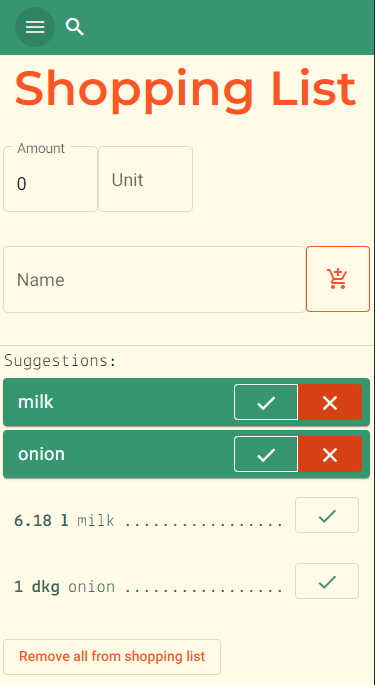
\includegraphics[scale=0.5]{pictures/mobile_suggestion.png}

\chapter{Felhasznált technológiák}
\section{Angular}
Egy TypeScript alapú Framework fejlesztői platform, ami a eredetileg a Google fejlesztette ki, de most már Open Source. Angular egy teljes újraírása a régi AngularJS-nek. Egyik legnagyobb előnye, hogy komponens alapú a keretrendszer, ami segítségével újra felhasználhatók a kódok. Single Page application felépítésével dinamikusan építi fel a weblapok a felhasználó interakciója szerint, ezzel is gyorsabb és kevesebb újratöltést igényel.

A tervezés során a Figmában is komponensekkel terveztem meg a weblap kinézetét mind telefonos mind desktopos formában. A komponenseket egyszerű létrehozni, valamint felhasználni a megfelelő helyeken. Ha magunknak akarjuk tervezni a komponenseket, akor sima HTML/CSS-el elérhető, amennyiben szeretnénk már egy népszerű és könnyen integrálható komponens bázist felhasználni, akkor az Angular Material használható.

\section{Angular Material}
Az Angular Material egy a Google által fejlesztett komponens bázis. Ez segít a fejlesztőknek már kész és modern dizájnos komponenseket egyszerűen felhasználni a projektekben. Ez elsősorban egy UI komponens dizájn könyvtár, ami integrálás után, csak importokkal már azonnal működik. A weblapján pedig példákkal és részletes dokumentációval felsorolja a létező felhasználható komponenseket és különböző változataikat.

Az én projektem is nagy részben ennek a könyvtárnak a komponenseit felhasználva épült fel. Csak pár helyen lett kiegészítve a már létező verzió, hogy illeszkedjek az eredeti tervekhez. Ezen felül az Theming azaz a projekt témája is az Angular Material alapján lett felépítve, hogy a komponenseknek könnyen meglehessen adni az alap színeket és tipográfia szabályokat.

\section{FireBase}
Mostmár a Google által fejlesztett webes és mobilos alkalmazások készítéséhez létrehozott platform. Manapság nagyon népszerű az egyszerűsített adatbázis felépítése valamint a könnyű és könnyen értelmezhető kezelő felülete, arról nem beszélve, hogy rengeteg dokumentáció létezik a fejlesztők számára.

Ebben a projektben elég sok helyen használom a Firebase funkcióit. Az egész weblap a Firebase Hosting felületéről működik. A GitHub-bal összekötve, ha a Main Branch-re van feltöltés, akkor a Firebase-en automatikusan deploy-oldódik az új production verzió.

A FireStore Database-t használom a weblap adatok tárolásához. Itt vannak eltárolva  receptek, felhasználók, felhasználókhoz különböző kollekciók és bevásárló lista meta adatok. A Cloud FireStore-on belül lehet beállítani az adatbázis Rule-okat.Ezt azt jelenti, hogy be lehet állítani, hogy különböző kollekciókat kik érhetik el, milyen tevékenységek vannak engedélyezve nekik, valamit, hogy milyen jogokkal milyen adatbázis műveleteket lehet csinálni. Amíg nem volt autentikáció beállítva és a development folyamat volt, akkor csak egy dátumot frissítettem, hogy meddig lehet az összes felhasználónak bármit csinálni. Viszont most már le van tiltva a receptek törése, valamint bejelentkezés nélküli lekérdezések is.

A FireBase Storage-ban tárolódnak a receptekből kimentett képek, amik az import során kerülnek az adatbázisba.

A legnagyobb biztonság érdekében a Firebase Auth-ot használom a weblap bejelentkezés és regisztrációs műveletekhez. Így lehetséges manuálisan regisztrálni majd bejelentkezni, viszont, akinek van Gmail fiókja annak lehetősége van egy lépésben azonnal regisztrálni és belépni annak segítségével.

A recept importálás és a bevásárlólista egy része a Firebase Cloud Function keresztül szerver oldalon fut. Ez nem csak olcsóbb, mivel szerver oldali lekérdezések ingyenesek a kliens oldalival szemben, hanem az importálás során felmerült problémát is megoldotta. Az importálásnál felmerűlt, hogy egy honlap nem lérdezhez le adatot egy másikról kliens oldalon keresztül, valamit a CORS okozta nehézségek elkerülése érdekében is hasznos volt. Azon kívül, mikor a bevásárló listába új alakanyag kerül, akkor egy trigger leful a szerver oldalon, ami segítségével állítjuk elő az ajánlóhoz a metaadatokat.

\section{PWA}
PWA azaz Progressive Web Application egy koncepció, amit követve lehetséges megbízható, alkalmazható és telepíthető webes applikációkat fejleszteni. Az alap szabályait követve a weblap platformspecifikus alkalmazássá alakítható. A PWA lehetővé teszi az alkalmazások használatát bárhol, bármikor, bármilyen eszközön. 

Ez eseten az Angular-t kellett kiegészíteni egy kevés plusz JavaScript kóddal, hogy ha az eszköznek nincs internet elérése, akkor a script alapján a localstorage-ba elmentett, valamint cache adatokat használja az indításhoz. Ezzel elérhető, hogy valamilyen szinten használható a weblap offline környezetben is.

\section{Schema.org}
A shema.org egy weblap, ami azért készűlt, hogy a közösség a központosított sémákat használja különböző weblapokon, e-mailekben, modellekben, adatbázisok tervezésében vagy sok más helyen. Sok különböző kódolással használható, de a legnépszerűbbek a JSON-LD, Microdata valamint a RDFa. Ezek a szótárak olyan entitásokat és kapcsolatokat írnak le, amik segítik a fejlesztők számára a megfelelő sémát kiválasztani. Tehát összességében, ez egy tervgyűjtemény.

A projektben fontos szerepet játszott a shema.org által biztosított “Recipe” séma feldolgozása és megértése, mivel a recept importálás más weblapokról ezen alapul. A jól felépített weblapok manapság tartalmaznak egy vagy több JSON-LD meta információt, amiben a weblapon jelenleg megjelenő adatok vannak eltárólva JSON formátumban a Shema.org szerinti felépítés alapján.

\section{Figma}
Egy  vektorgrafikus szerkesztő, ahol web prototípusokat lehet tervezni. Ez legfőképp webalapú, de letölthető desktopos verziója is. A program képes a tervezett lapok élő tükrözésére akár saját telefonon az applikáción keresztül, vagy csak az emuláló felületen keresztül is. A figma egy modern dizájn tervező felület, ahova egyszerűen integrálni lehet a material design stílust és alap komponenseket, ezzel is segítve az Angular component szerű gondolkodást. Másik nagy előnye, hogy interaktívvá lehet tenni a tervezés során a gombokat, komponenseket. Valamint a kész dizájnoknak meglehet nézni a pontos CSS stílus kódját is, ezzel is segítve a konkrét kódolás folyamatát.

Sokat segített a tervezésben, mivel a kész material design komponenseket tudtam próbálgatni anélkül, hogy először mélyebben tanulmányoznám az Angular felépítését. Az egységes dijájn és téma felépítésében pedig segített konzisztensnek maradnom. Ez igaz mint a színekre, mind a tipográfiára.


\chapter{A rendszer magas szintű áttekintése}
Ebben a fejezetben fogom leírni a különböző fontosabb funkciókról a részletesebb felépítését és tudnivalókat.

\section{Recept importálás}
A moduláris felépítés miatt ezt több al részre szedem.

\subsection{FetchUrlData}
asd
\subsection{JsonLdExtractor}
asd
\subsection{SeparateIngredients}
asd
\subsection{ImageDownloader} 
asd
\subsection{CalorieCalculator}
asd
\section{Kliens oldali adatbázis műveletek}
Services...

\section{Bevásárlólista ajánló}
trigger és működés

%TODO: more?

\chapter{Architektúra}
\section{asd}


\chapter{Adatmodellek}
\section{asd}


%\chapter{Fontosabb kód részek és ismertetései}
%\section{asd} -> A rendszer magas szintű áttekintése


\chapter{Tesztelés}
\section{asd}


\chapter{Továbbfejlesztési lehetőségek}
\section{asd}



\chapter*{Nyilatkozat}
%Egy üres sort adunk a tartalomjegyzékhez:
\addtocontents{toc}{\ }
\addcontentsline{toc}{section}{Nyilatkozat}
%\hspace{\parindent}

% A nyilatkozat szövege más titkos és nem titkos dolgozatok esetében.
% Csak az egyik tipusú myilatokzatnak kell a dolgozatban szerepelni
% A ponok helyére az adatok értelemszerűen behelyettesídendők es
% a szakdolgozat /diplomamunka szo megfeleloen kivalasztando.


%A nyilatkozat szövege TITKOSNAK NEM MINŐSÍTETT dolgozatban a következő:
%A pontokkal jelölt szövegrészek értelemszerűen a szövegszerkesztőben és
%nem kézzel helyettesítendők:

\noindent
Alulírott \makebox[4cm]{\dotfill} szakos hallgató, kijelentem, hogy a dolgozatomat a Szegedi Tudományegyetem, Informatikai Intézet \makebox[4cm]{\dotfill} Tanszékén készítettem, \makebox[4cm]{\dotfill} diploma megszerzése érdekében.

Kijelentem, hogy a dolgozatot más szakon korábban nem védtem meg, saját munkám eredménye, és csak a hivatkozott forrásokat (szakirodalom, eszközök, stb.) használtam fel.

Tudomásul veszem, hogy szakdolgozatomat / diplomamunkámat a Szegedi Tudományegyetem Informatikai Intézet könyvtárában, a helyben olvasható könyvek között helyezik el.

\vspace*{2cm}

\begin{tabular}{lc}
	Szeged, \today\
	\hspace{2cm} & \makebox[6cm]{\dotfill} \\
	             & aláírás                 \\
\end{tabular}


\vspace*{4cm}

%A nyilatkozat szövege TITKOSNAK MINŐSÍTETT dolgozatban a következő:

\noindent
Alulírott \makebox[4cm]{\dotfill} szakos hallgató, kijelentem, hogy a dolgozatomat a Szegedi Tudományegyetem, Informatikai Intézet \makebox[4cm]{\dotfill} Tanszékén készítettem, \makebox[4cm]{\dotfill} diploma megszerzése érdekében.

Kijelentem, hogy a dolgozatot más szakon korábban nem védtem meg, saját munkám eredménye, és csak a hivatkozott forrásokat (szakirodalom, eszközök, stb.) használtam fel.

Tudomásul veszem, hogy szakdolgozatomat / diplomamunkámat a TVSZ 4. sz. mellékletében leírtak szerint kezelik.

\vspace*{2cm}

\begin{tabular}{lc}
	Szeged, \today\
	\hspace{2cm} & \makebox[6cm]{\dotfill} \\
	             & aláírás                 \\
\end{tabular}





\chapter*{Köszönetnyilvánítás}
\addcontentsline{toc}{section}{Köszönetnyilvánítás}

Ezúton szeretnék köszönetet mondani \textbf{X. Y-nak} ezért és ezért \ldots


%% Az itrodalomjegyzek keszitheto a BibTeX segedprogrammal:
%\bibliography{diploma}
%\bibliographystyle{plain}

%VAGY "kézzel" a következő módon:

\begin{thebibliography}{9}
	%10-nél kevesebb hivatkozás esetén

	%\begin{thebibliography}{99}
	% 10-nél több hivatkozás esetén

	\addcontentsline{toc}{section}{Irodalomjegyzék}

	%Elso szerzok vezetekneve alapjan ábécérendben rendezve.


	%folyóirat cikk: szerzok(k), a folyóirat neve kiemelve,
	%az evfolyam felkoveren, zarojelben az evszam, vegul az oldalszamok es pont.
	\bibitem{Gischer}
	J. L. Gischer,
	The equational theory of pomsets.
	\emph{Theoret. Comput. Sci.}, \textbf{61}(1988), 199--224.

	%könyv (szerzo(k), a könyv neve kiemelve, utana a kiado, a kiado szekhelye, az evszam es pont.)
	\bibitem{Pin}
	J.-E. Pin,
	\emph{Varieties of Formal Languages},
	Plenum Publishing Corp., New York, 1986.





\end{thebibliography}




\end{document}
